

El presente recurso pretende explicar las unidades didácticas del bloque de Análisis matemático referidas a las funciones y a la representación de las mismas. Las finalidades con las que éste ha sido creado son dos, claramente diferenciadas:
\begin{itemize}
	\item Dada la fórmula o ecuación de una función, saber representarla gráficamente.
	\item Dada la fórmula o ecuación de una función, analizarla estudiando todas sus características.
\end{itemize}
Sin embargo, antes de poder centrarnos en el análisis de funciones, haremos un breve repaso del temario dado en 1º de Bachillerato acerca de las mismas.\\

\begin{itemize}
	\item \textbf{Organiza tus ideas}
	\begin{figure}
		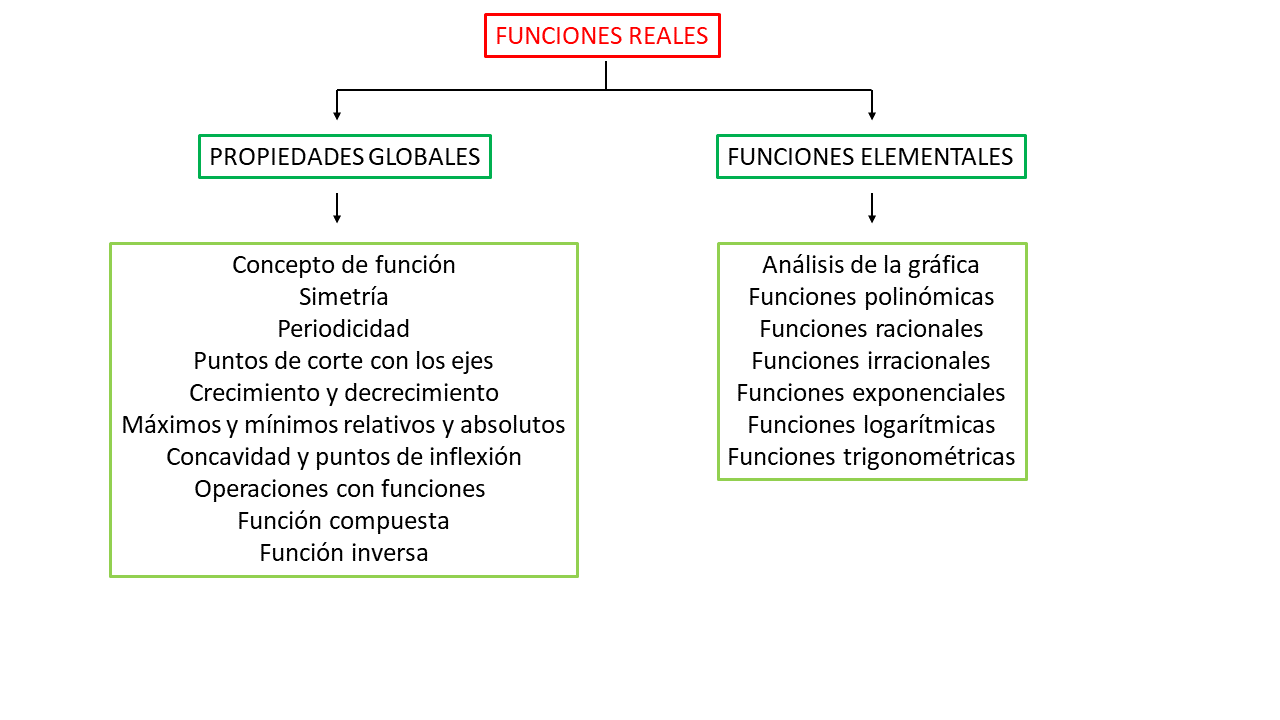
\includegraphics[width=30cm, height=25cm]{samples/ideas.png}
		\centering
	\end{figure}
\end{itemize}
